\documentclass[conference]{IEEEtran}
\usepackage{graphicx}
\usepackage{booktabs}
\usepackage{array}
\usepackage{xurl}
\usepackage[hidelinks]{hyperref}
\hyphenation{STRATA Process-Heal}

\title{STRATA: A Process-Mining Framework That Finds HVAC Faults in a Building's Own Trend Data and Says Where They Are}

\author{\IEEEauthorblockN{Yassh Singh}
\IEEEauthorblockA{Thompson Rivers University, Kamloops, Canada\\
Undergraduate Research Experience Award Program (U-REAP) 2026\\
Supervisors: Dr.\ Anthony Aighobahi and Dr.\ Mridula Sharma\\
singhy21@mytru.ca}}

\begin{document}
\maketitle

\begin{abstract}
Faults and poor control in heating, ventilation and air-conditioning (HVAC) equipment waste 15 to 30 percent of a commercial building's energy, and most of them go unnoticed. The fault-detection tools buildings already have either catch only the faults somebody wrote a rule for or flag anomalies nobody can act on. This paper presents STRATA, a framework that reads the one-minute trend data a building already records, learns what healthy operation looks like from one fault-free period, and scores each new day with eight checks. A check may raise an alarm only when it beats its own false-alarm rate, measured on fault-free days it never trained on. Every alarm names the unit, the part affected and the evidence. The framework is built with process mining. The building's sensor data is turned into a log of events along the control sequence; models of normal operation are discovered from that log for each terminal unit and for the whole unit, and those models give every alarm its location. On the five main systems in the public benchmark datasets from Lawrence Berkeley National Laboratory, STRATA detected 158 of 175 seeded faults, most on the first day, with 26 false-alarm days in 480 held-out fault-free days, and named the correct terminal unit in 37 of 50 checkable cases and a wrong one in none. A new building is onboarded by writing one configuration file; the code does not change. We describe each stage of the framework in plain terms, show what it did on the benchmarks, and set out how it would be deployed on a real building such as one at Thompson Rivers University as the next step. STRATA is the first stage of ProcessHeal, a programme whose goal is a building that detects, locates, diagnoses and corrects its own faults.
\end{abstract}

\begin{IEEEkeywords}
HVAC, fault detection, process mining, building automation, event logs, explainable alarms
\end{IEEEkeywords}

\section{Introduction}

A building operator today finds a fault in two ways: someone complains that a room is too hot, or the operator notices by eye that a line on a trend graph has drifted from where it usually sits. Both find the fault late, both depend on someone happening to look, and neither says which piece of equipment is responsible. Buildings account for about a third of energy-related carbon emissions \cite{unep2025gsr}, HVAC accounts for up to half of a building's energy use \cite{bi2024aihvacreview}, and faults and poor control that nobody sees waste 15 to 30 percent of a commercial building's energy \cite{katipamula2005fddreview1}. A study of more than 60,000 pieces of HVAC equipment in commercial buildings found 40 percent of air handlers in a faulted state on any given day, in buildings that already had automation systems with alarms \cite{crowe2023faultprevalence}.

The tools that exist fall into two groups. Commercial building-automation systems ship libraries of rules written in advance: if the valve is commanded closed but water still flows, raise an alarm \cite{schein2006apar}. These are clear and need no training data, but they catch only the faults somebody wrote a rule for. Research methods based on machine learning catch more, but they output an anomaly score: a number that says today is unusual, without saying where or why \cite{bi2024aihvacreview}. An operator cannot write a work order from a number.

This paper presents STRATA, a framework that takes the strength of each. It learns what normal looks like from the building's own healthy operation, so it is not limited to pre-written rules. Every alarm it raises names the equipment, the physical relationship that broke and the evidence, so an operator can act on it. It is built with process mining, a method for discovering a model of a process from a log of events and checking later behaviour against that model \cite{vanderaalst2016processmining}. To our knowledge, process mining has not been applied to HVAC fault detection before; the surveys of the field contain no such entry \cite{bi2024aihvacreview,brzychczy2025pmsensorreview}.

This report is written so that a reader who has not seen the full research paper can understand how the framework works and what it does. Section~\ref{sec:framework} walks through the framework stage by stage. Section~\ref{sec:results} shows what it did on public benchmark data. Section~\ref{sec:deploy} describes how it would be deployed on a real building. Section~\ref{sec:limits} states the limits. The full evaluation, with every experiment and its outcome, is in the long paper and the public repository.\footnote{\url{https://github.com/iyassh/strata}}

\section{The Framework, Stage by Stage}
\label{sec:framework}

Figure~\ref{fig:framework} shows the framework. The top half runs once per building, on one fault-free period of data, and produces the models and the thresholds. The bottom half runs every day. The stages below follow the figure from left to right. Table~\ref{tab:terms} defines the terms they use.

\begin{table}[t]
\centering
\caption{Terms used in this paper.}
\label{tab:terms}
\small
\setlength{\tabcolsep}{4pt}
\begin{tabular}{@{}>{\raggedright\arraybackslash}p{0.24\columnwidth}>{\raggedright\arraybackslash}p{0.72\columnwidth}@{}}
\toprule
Term & Meaning here \\
\midrule
Trend data & The minute-by-minute sensor and actuator values a building-automation system (BAS) records. \\
Unit & An air handler or rooftop unit that serves several zones. \\
Zone & A room or group of rooms served by one terminal unit. \\
Terminal unit & The box that serves one zone: its damper, reheat valve and, in some designs, a small fan. \\
Device & A terminal unit; the word used in the names of the device level and the device conformance check. \\
Event & One thing that happened at one time, such as ``cooling started at 09:14''. \\
Event log & All the events of all the days, one case per day. \\
Process model & A graph, discovered from the log, of the states a terminal unit or a unit passes through on a normal day and in what order. \\
Conformance & How well one day's events fit the process model. \\
Check & One of the eight tests run on each day; seven can raise an alarm, the eighth only supports one. \\
Seeded fault & A fault written into a simulation on purpose, so the right answer is known. \\
Scenario & One simulated run, usually a year, that contains one seeded fault. \\
Held-out days & Fault-free days kept aside and used only to measure how often each check gives a false alarm. \\
Measured false-alarm rate & The false-alarm rate of a check, measured on the held-out days, and reported with every alarm the check raises. \\
\bottomrule
\end{tabular}
\end{table}

\begin{figure*}[t]
\centering
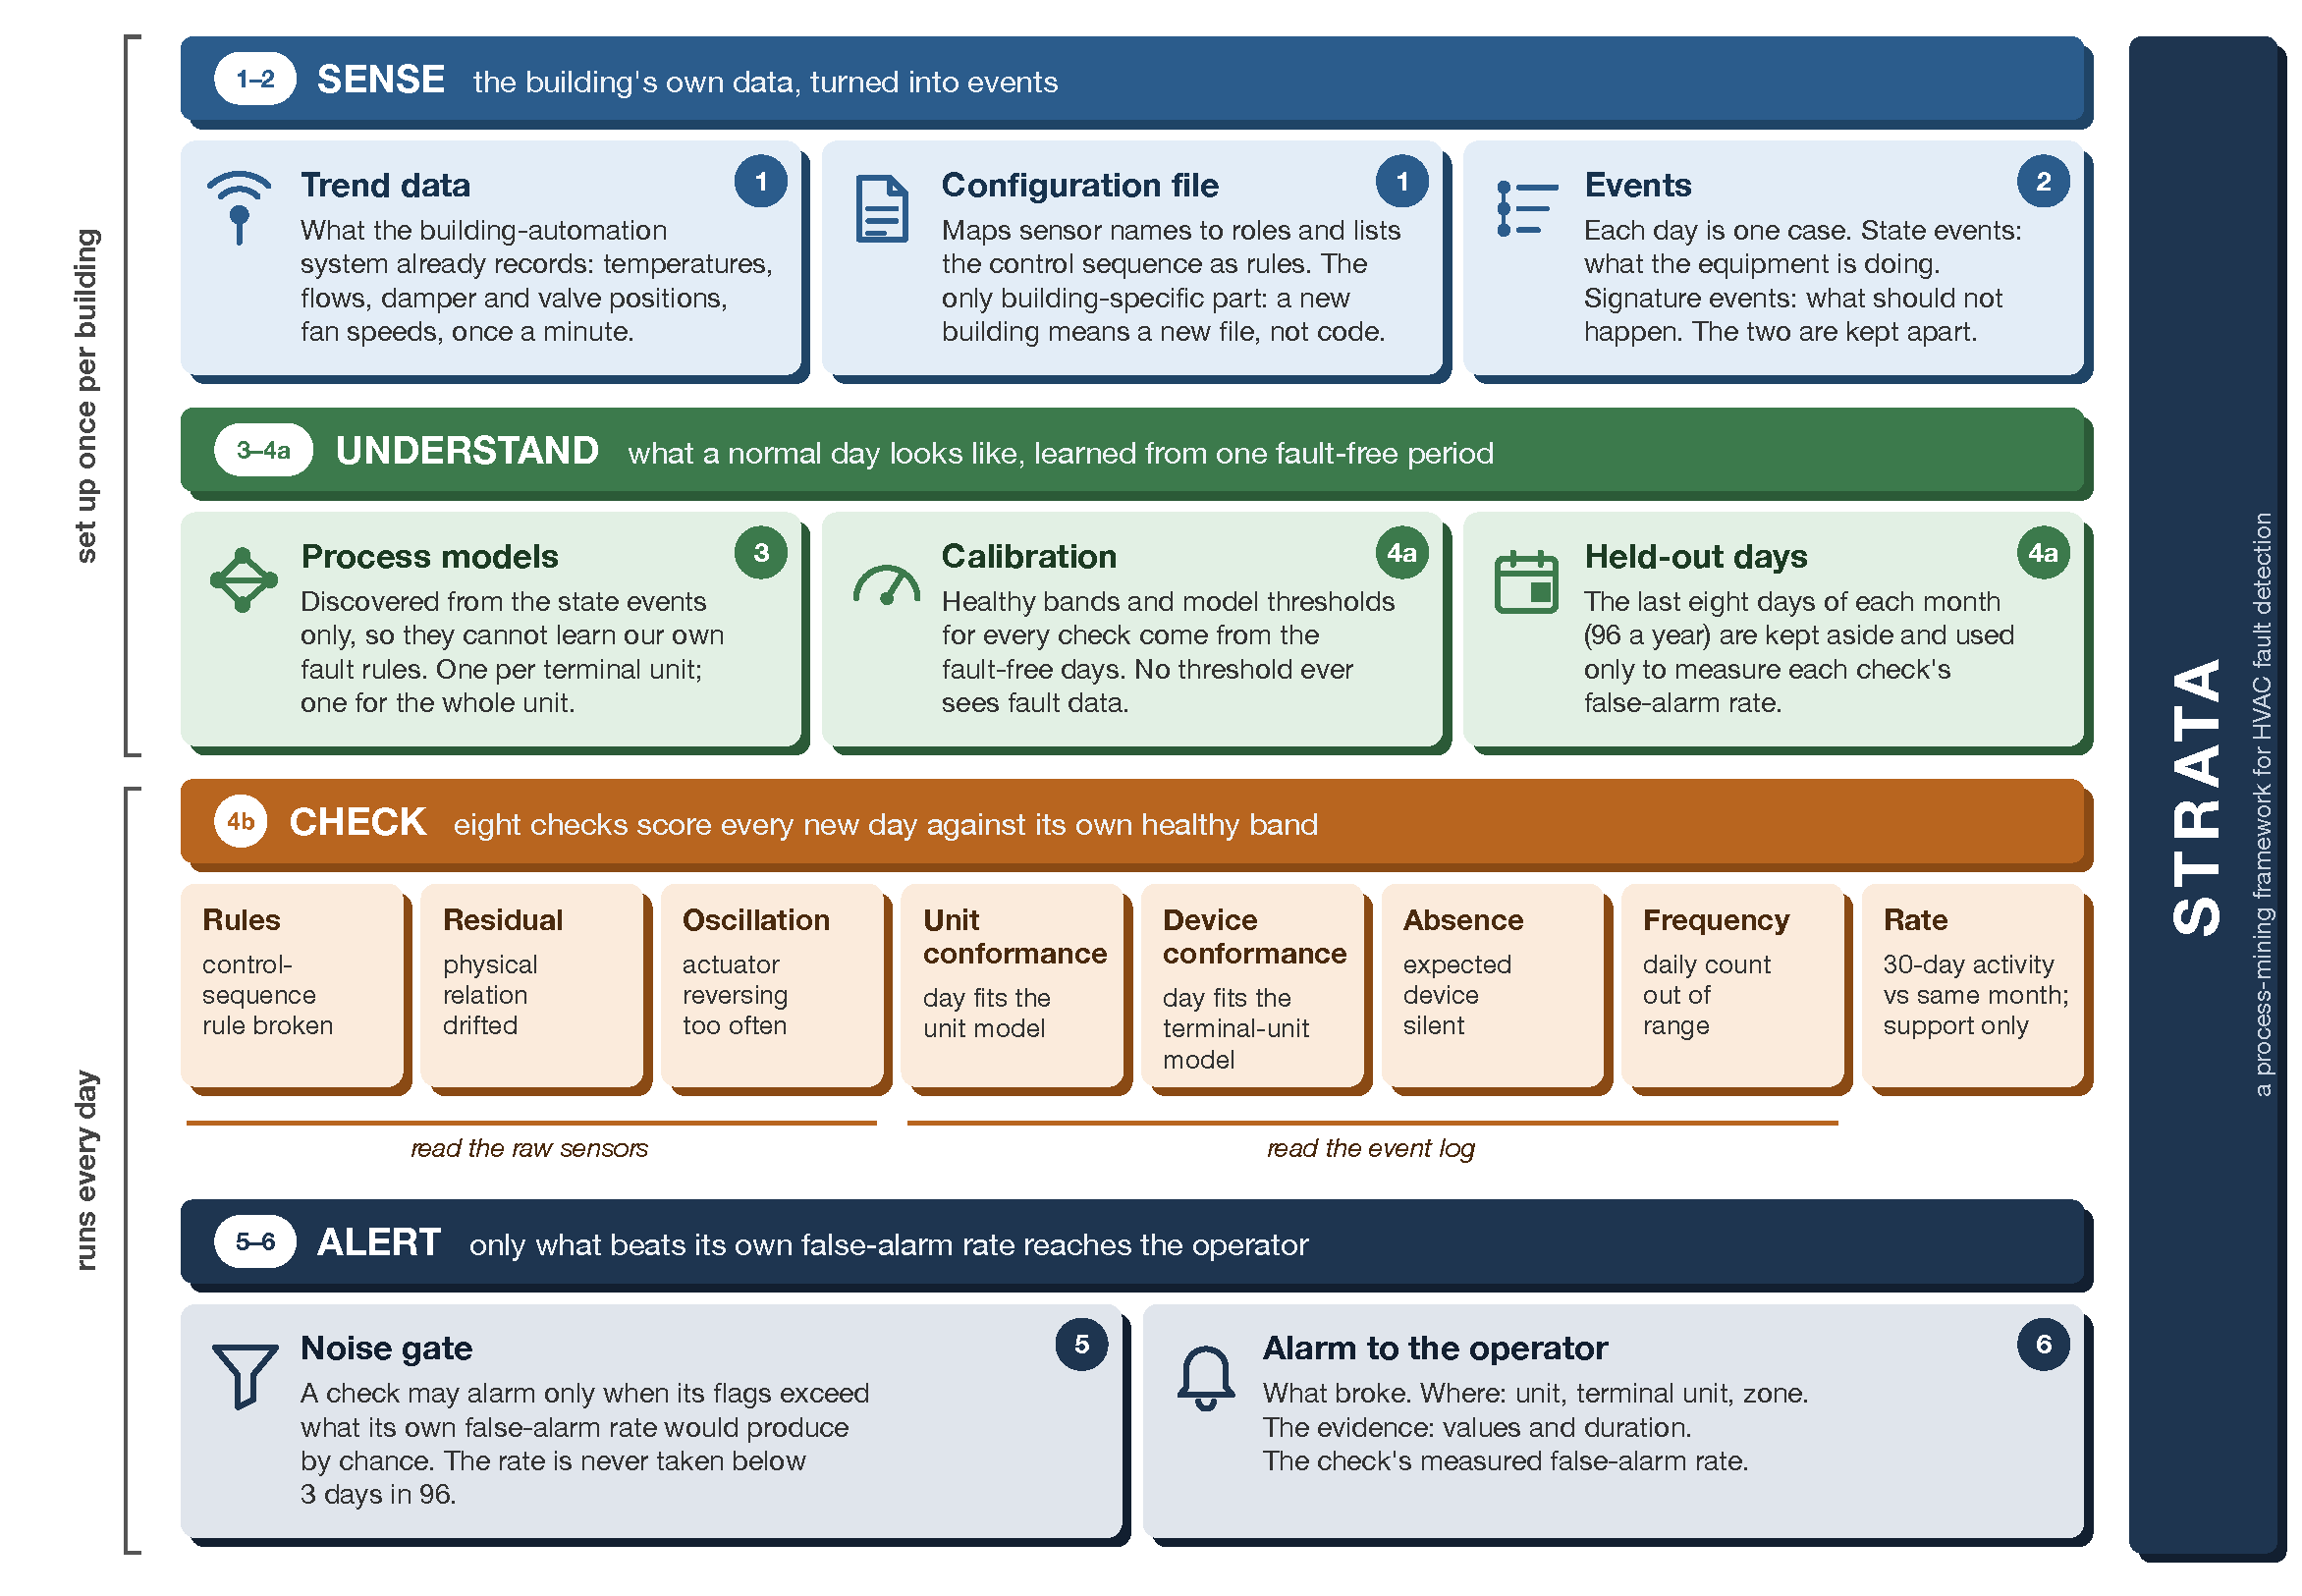
\includegraphics[width=0.98\textwidth]{../figures/strata_framework_report.pdf}
\caption{The STRATA framework. Training (top) runs once per building on one fault-free period: the trend data is turned into events, process models of a normal day are discovered from the state events, and the eight checks are calibrated, with their false-alarm rates measured on held-out days. Deployment (bottom) runs every day: the new day is scored by the eight checks, the noise gate passes only alarms that beat the check's own false-alarm rate, and what passes reaches the operator with a fault name, a location, the evidence and the check's measured false-alarm rate. The numbers are the stages of Section~\ref{sec:framework}; 4a and 4b are the two halves of Stage 4, and the new day's box is Stage 2 run again.}
\label{fig:framework}
\end{figure*}

\subsection{Stage 1: the building's data and one configuration file}

The input is the trend data a building-automation system already records: temperatures, flows, pressures, damper and valve positions, fan speeds, usually once a minute. STRATA does not need new sensors. It needs one fault-free period of that data, ideally a year so that every season is seen, and one configuration file.

The configuration file is the only thing that is specific to a building. It has two parts. The first maps the building's sensor names to the roles the framework understands: this column is the supply-air temperature, that one is a zone's damper position. The second lists the control sequence for this type of equipment as rules, taken from the design documents and the ASHRAE Guideline 36 sequences \cite{ashrae2021guideline36}. These rules come in two families. State rules say when the unit is occupied and when it is in heating or cooling mode. Signature rules say which relationships must hold, such as no flow through a closed valve.

Onboarding a new building means writing this file; the pipeline code does not change. On the benchmarks, configuring the second equipment type took about one and a half hours. Two of the five main benchmark systems were configured before any fault data was opened, so nothing in them could have been tuned to the faults.

\subsection{Stage 2: turning sensor data into events}

Process mining works on event logs, not on sensor curves, so the first thing the framework does with the data is turn the minute-by-minute values into events along the control sequence. Each day is one case. An event is something like ``fan started at 06:02'', ``cooling became active at 09:14'' or ``outside air became cool enough for free cooling at 11:40''. The configuration's rules produce them: a state rule for operating mode fires an event when the mode changes, and a signature rule fires one when the relationship it guards is broken.

There are two kinds of events, and keeping them apart is one of the framework's main ideas. \emph{State events} describe what the equipment is doing, with no judgement attached. \emph{Signature events} describe something that should not happen, such as ``water flowing through a valve that is commanded closed''. Only the state events are allowed into the next stage, model discovery. If the signature events were allowed in, the discovered model would simply learn our own fault rules and later ``detect'' them, which would be circular. We measured this. On one system, letting signature events into discovery raised the unit conformance check's apparent detection from 1.8 to 5.2 percent of fault days, and every added day was the model re-finding a rule we had written.

\subsection{Stage 3: discovering what normal looks like}

From the state-event log of the fault-free period, the framework discovers process models of a normal day with a standard process-mining algorithm, the inductive miner \cite{leemans2013inductiveminer}. It does this at two levels; the levels are the strata the name refers to. The \emph{device} level has one model per terminal unit, describing the normal day of that terminal unit's damper and reheat valve. The \emph{unit} level has one model for the air handler's whole daily cycle. Each model is a graph of the states the device or unit passes through and the order it passes through them (a Petri net, in process-mining terms). A third, cross-building level was built only to test whether a model transfers between buildings. It is not part of the daily detector.

These models do two things in the framework. First, they give every alarm its location: because events and models exist per terminal unit, an alarm raised by one zone's device model is an alarm about that zone. Second, during development they surfaced invariants of normal operation, things that were always true on healthy days, which we then wrote down as rules in the configuration. What the models do not do, which we tested, is detect faults by themselves (Section~\ref{sec:results}).

\subsection{Stage 4: eight checks, each calibrated on the fault-free period}

Each day is scored by eight checks. Three of them read the raw sensor data:
\begin{itemize}
\item \emph{Rules}: a control-sequence rule was broken, such as flow through a closed valve, or a zone's airflow far from its setpoint while occupied.
\item \emph{Residual}: a physical relationship that must hold in a known mode has drifted out of its healthy band. With the cooling coil off, the supply-air temperature should equal the mixed-air temperature plus the small rise from the fan; if it does not, a sensor is biased or a coil is leaking.
\item \emph{Oscillation}: an actuator reversed direction far more often than it does on healthy days, the sign of an unstable control loop.
\end{itemize}
Four of them read the event log:
\begin{itemize}
\item \emph{Unit conformance} and \emph{device conformance}: how well today's sequence of events fits the discovered model of the unit or of the terminal unit. A day fits poorly when, for example, cooling starts before the fan, an order the fault-free period never showed.
\item \emph{Absence}: a device that is active on every healthy scheduled day produced no events on a scheduled day.
\item \emph{Frequency}: a daily count, such as the number of heating episodes, left its healthy range.
\end{itemize}
The eighth, a \emph{rate} check, looks at the last 30 days and compares how many of them a mode was active with the same calendar month of the fault-free year. It may support an alarm but never raise one alone, because on one system it added false alarms.

Every threshold in every check comes from the fault-free period only. The year is split by the calendar: the last eight days of each month (96 days in a year) are held out and never used for setting anything; they exist only to measure how often each check gives a false alarm. The remaining days set the healthy bands and train the models. No threshold ever sees fault data, and no threshold sees the days on which its false-alarm rate is later reported.

\subsection{Stage 5: the noise gate}

A check is allowed to raise an alarm on a scenario only when the number of days it flagged is too large to be explained by its own false-alarm rate. The test is a simple probability calculation, the same one used for coin tosses. Suppose a check wrongly flags three of 96 held-out fault-free days. Flagging forty of 365 days in a scenario is then far beyond what chance would give, and the check may alarm; flagging five is not, and it may not. The floor is never set below three days in 96, so a check cannot claim a zero false-alarm rate it has not earned.

On the benchmarks this test is applied once per check per scenario, to decide whether the check is credited with the detection; the first day the credited check flagged is the day of the alarm. In a building there is no scenario, only days. A check whose false-alarm rate has been measured on the held-out days, and which stayed quiet on the rest of the fault-free period (step 3 of Table~\ref{tab:deploy}), would report each day it flags, together with that rate. That is what we mean by a measured false-alarm rate: before the first alarm is trusted, the operator knows how often each check cries wolf.

\subsection{Stage 6: the alarm the operator receives}

What survives the gate reaches the operator with four things: what broke, where, the evidence, and the check's measured false-alarm rate. Figure~\ref{fig:alarm} shows one from the benchmarks, as the framework printed it. The fault seeded was a zone damper stuck at 80 percent open. The alarm names the zone, names the terminal unit, states that the primary airflow is 515 cubic feet per minute above its setpoint and has been for twelve hours while occupied, reports the damper position of 0.80 against a normal 0.32, and tells the operator that the rules check gave zero false alarms on the 96 held-out fault-free days. It was raised on the first day of the fault.

\begin{figure}[t]
\footnotesize
\begin{verbatim}
STRATA alarm -- series fan-powered unit,
               2018-01-01 (day 1 of the fault)
 what     zone primary-air flow not tracking
          its setpoint           [check: rules]
 where    terminal unit TU_S, zone S
 evidence 715 CFM measured against a 200 CFM
          setpoint, a 515 CFM excess, held for
          720 min while occupied; damper 0.80,
          fault-free same-day value 0.32
 rate     rules check: 0 false-alarm days on
          the 96 held-out fault-free days
 truth    zone-S damper stuck at 80%: location
          and symptom correct, caught on day 1
\end{verbatim}
\caption{One alarm from the benchmark. Every value is taken from the framework's recorded output and the benchmark data; the last line is the answer key, not part of the alarm. The alarm names the symptom and the location; it does not claim the root cause.}
\label{fig:alarm}
\end{figure}

\section{What It Did on Public Benchmark Data}
\label{sec:results}

We evaluated the framework on the public HVAC fault-detection datasets from Lawrence Berkeley National Laboratory \cite{granderson2023lbnlfdddata}. Each simulated dataset is one-minute data for one type of equipment, recorded once fault-free and once per seeded fault: a stuck damper, a biased sensor, a fouled coil, a leaking valve, an unstable controller. The five main systems have a full year of data; the two rooftop datasets are shorter. Because the faults are seeded, we know exactly which fault is in which file.

Table~\ref{tab:systems} lists the seven datasets: air handlers that serve many zones through one duct (single-duct) or through separate hot and cold ducts (dual-duct), two kinds of fan-powered terminal unit, a fan coil unit that serves one room, and two rooftop units. Six are simulated; one is a measured year from a real rooftop unit. The five main systems carry the headline numbers. The sixth, a simulated rooftop unit, is the only one that records the refrigerant side and was used for those faults. The measured unit has 182 clean days and one fault case, so it gives a false-alarm rate and no detection count.

\begin{table}[t]
\centering
\caption{The seven LBNL datasets. ``Scored'' is the number of seeded faults evaluated; ``detected'' those the framework caught; ``false alarms'' the held-out fault-free days on which it alarmed. $^{\dagger}$13 after an audit attributed one detection to a dataset defect rather than to the fault. The text's 158 counts it; the audited total is 157. The two rooftop datasets are shorter, so the same held-out rule gives fewer held-out days.}
\label{tab:systems}
\small
\setlength{\tabcolsep}{5pt}
\begin{tabular}{@{}lrrl@{}}
\toprule
System & scored & detected & false alarms \\
\midrule
Single-duct air handler & 14 & 14$^{\dagger}$ & 1 of 96 \\
Parallel fan-powered unit & 30 & 26 & 8 of 96 \\
Series fan-powered unit & 29 & 25 & 9 of 96 \\
Dual-duct air handler & 55 & 50 & 3 of 96 \\
Fan coil unit & 47 & 43 & 5 of 96 \\
Rooftop unit (simulated) & 24 & 20 & 0 of 28 \\
Rooftop unit (measured) & 1 case & --- & 3 of 49 \\
\bottomrule
\end{tabular}
\end{table}

\subsection{Detection and false alarms}

Across the five main systems the framework detected 158 of 175 seeded faults, with 26 false-alarm days in 480 held-out fault-free days, between 1 and 9.4 percent per system. The median time from the start of a fault to its first alarm was one day. On the real rooftop unit the false-alarm rate was 3 of 49 held-out days. Sixteen of the 158 came from an audit that mapped every recorded column the first configurations had left unread. The 17 faults it missed are all coil fouling. For some coils every seeded severity was missed, because the recorded sensor values stay inside every healthy band; nothing that reads only those values could see them. On the one dataset that records the refrigerant side, the framework caught every fouling severity.

\subsection{Where the alarm points}

On the two fan-powered systems, where each unit serves four terminal units, the alarm named the correct terminal unit in 37 of the 50 checkable cases (the detections before the column audit whose seeded fault sat in one terminal unit), named none in 13 (the alarm named the unit but no terminal unit), and named a wrong one in none. Over all 158 detections the rule carrying the alarm pointed at the right part of the equipment (which coil, which fan, which damper, which terminal unit) in 83 percent of cases and at the exact seeded component in 69 percent. The alarm names the symptom and the place. It does not name the root cause: a first diagnosis layer we tested improved the pointing a little but did not reach the targets we had set for it, so we make no diagnosis claim.

\subsection{Against two baselines}

Against principal component analysis, a standard statistical method applied to the raw sensors, the framework detected 64 of 73 shared scenarios to the baseline's 61, a difference too small to be sure of. The baseline cannot name the terminal unit. Against the Guideline 36 fault rules that commercial systems run, implemented by an independent open-source library and scored under the same gate, the framework was level on the single-duct air handler and detected three times as many faults on the terminal units, because it reads the per-zone sensors the rules do not (Table~\ref{tab:g36}). We had predicted that STRATA would detect at least as many faults at no higher false-alarm rate on every system. It did not: on the air handler it was level, and on the terminal units its extra coverage cost eight and nine false-alarm days against the rules' none.

\begin{table}[t]
\centering
\caption{STRATA against the Guideline 36 fault rules on the three systems both were run on, under the same gate. ``Found'' is seeded faults detected; ``false'' is false-alarm days among the held-out days. The single-duct count is the audited 13 of Table~\ref{tab:systems}.}
\label{tab:g36}
\footnotesize
\setlength{\tabcolsep}{3pt}
\begin{tabular}{@{}lcccc@{}}
\toprule
 & \multicolumn{2}{c}{STRATA} & \multicolumn{2}{c}{Guideline 36 rules} \\
System & found & false & found & false \\
\midrule
Single-duct air handler & 13 of 14 & 1 of 96 & 12 of 14 & 1 of 96 \\
Parallel fan-powered unit & 26 of 30 & 8 of 96 & 8 of 30 & 0 of 96 \\
Series fan-powered unit & 25 of 29 & 9 of 96 & 9 of 29 & 0 of 96 \\
\bottomrule
\end{tabular}
\end{table}

\subsection{What process mining contributes}

We began with the hypothesis that the discovered process models would detect the faults themselves. They did not. Over 199 scenarios on six systems (the 175 plus the 24 on the simulated rooftop unit), no fault was caught by the conformance checks alone, and on the model's best scenario a one-line hand-written rule flagged more fault days than the model did. What process mining contributes is the structure: the per-terminal-unit models give every alarm its location, the models surfaced invariants that became detection rules (for example, that the air handler's heating never runs on an occupied workday), and on the fan-powered units the frequency check, which counts events in the log, and the oscillation check are the only ones that see the unstable-controller faults. Process mining helps to get detection but is not detecting on its own. That finding came from pre-registered tests, with the refuting result written down before each one was run, and it is why the framework is built the way it is.

\subsection{Under noisier data}

Simulated data is cleaner than a real building's. To check that this had not flattered the results, we injected sensor noise, logging that records a value only when it changes, as many real systems do, gaps in the record, and shifted schedules into the fault-free year and every fault file, re-fitted, and re-scored all five systems. Before running this test we had set a limit of 10 false-alarm days in 96. Every system stayed under it, with the worst count at 7 of 96, and each condition cost at most one detection per system.

\section{How It Would Be Used in a Real Building}
\label{sec:deploy}

Nothing in this section has been done; it is the next step. We describe it because it is the point of the framework, and we use Thompson Rivers University (TRU) as the example because the work was done there and a trial there is planned. A 2022 energy study of the Campus Activity Centre lists an air-handling unit serving variable-air-volume boxes (terminal units), fan coil units and five rooftop units, all of them equipment types the framework has been evaluated on, with nearly every system logging on an Automated Logic brand building-automation system \cite{ses2022cacstudy}. Table~\ref{tab:deploy} gives the steps.

\begin{table}[t]
\centering
\caption{Deploying the framework on a building. Steps 1 to 3 are the training half of Figure~\ref{fig:framework}; step 4 is the deployment half.}
\label{tab:deploy}
\small
\setlength{\tabcolsep}{3pt}
\begin{tabular}{@{}>{\raggedright\arraybackslash}p{0.21\columnwidth}>{\raggedright\arraybackslash}p{0.37\columnwidth}>{\raggedright\arraybackslash}p{0.36\columnwidth}@{}}
\toprule
Step & What is needed & What comes out \\
\midrule
1. Collect & A fault-free period of trend data from the building-automation system at its own sampling rate; a year is best, but 182 days was enough to measure a false-alarm rate on the rooftop unit & The healthy baseline \\
2. Configure & The point list (every sensor and actuator the system records), mapped to the framework's roles; the control sequence as rules; every recorded point mapped or excluded with a reason & The configuration file, the only file specific to the site \\
3. Confirm silence on the fault-free period & Run the detector on the fault-free period; it must raise no alarm there, so any rule that fires is fixed or removed first & A detector whose false-alarm rate is measured on this building's own held-out days \\
4. Operate & Each day's data & Alarms naming the unit, the part affected and the evidence, each with the check's measured false-alarm rate \\
\bottomrule
\end{tabular}
\end{table}

Three things decide whether it works on a real building, and all three are checked before the first alarm is trusted. The fault-free period must really be fault-free: one faulty day in it can move a band edge, so the period is audited first. The configuration must read every recorded point: on the benchmarks, an audit of every column recovered sixteen faults that the first configuration had missed. And the silence step must be run at the building's own sampling rate, because thresholds set on one-minute data do not transfer to fifteen-minute data. What the operator would then get is a daily list of alarms in the form of Figure~\ref{fig:alarm}, each naming the unit and the part affected, with the false-alarm rate of each check already known.

\section{Limits}
\label{sec:limits}

\begin{itemize}
\item Every detection result above comes from simulated data, and simulated years are cleaner than real ones. The one real building so far supports a false-alarm rate, not a detection rate.
\item Two scoring choices were made after we saw their effect. The rate check was demoted to support-only. The two conformance checks had their thresholds set on the same days later used to measure their false-alarm rates; we re-set them on separate days, which raised two reported rates.
\item Slowly developing faults are caught late, up to 114 days for two fouling cases.
\item The benchmarks seed equipment and sensor faults, not the schedule and override faults that are most common in real buildings, such as a unit left in manual or a schedule left in holiday mode.
\item The alarm names the symptom and the location, not the cause. Diagnosis and automated correction are the later stages of ProcessHeal, and would need active tests and an operator study before any automated action.
\end{itemize}

\section{Conclusion}

STRATA turns the trend data a building already records into alarms an operator can act on: it learns normal operation from one fault-free period, checks each day against physics and against discovered process models, lets through only alarms that beat a measured false-alarm rate, and names the unit, the part and the evidence. On the five main benchmark systems it detected 158 of 175 seeded faults, with the false-alarm rate of every check measured on held-out days and reported with each alarm, and, in the 50 cases where this could be checked, never named a wrong terminal unit. It is onboarded with a configuration file rather than new code. Process mining gives the framework its structure and the location on every alarm; the detecting is done by the calibrated checks. The next step is a live trial on a real building, and TRU's own campus is the intended place to run it.

\section*{Acknowledgements}
The author thanks Dr.\ Anthony Aighobahi and Dr.\ Mridula Sharma for their supervision, and the U-REAP program for its support.

\bibliographystyle{IEEEtran}
\bibliography{../references}
\end{document}
